%
\documentclass[10pt]{article}

% The usual packages
\usepackage{booktabs}
\usepackage{array}
\usepackage{subcaption}


\usepackage{fullpage}
\usepackage{breakcites}
\usepackage{setspace}
\usepackage{endnotes}
%\usepackage{float} % can't use with floatrow
\usepackage{amsmath}
\usepackage{amsfonts}
\usepackage{amssymb}
\usepackage{rotating}
\usepackage{longtable}
\usepackage{microtype}
\usepackage{graphicx}
\usepackage{hyperref}
%\usepackage[usenames,dvipsnames]{color}
\usepackage{url}
\usepackage{natbib}
\usepackage{framed} 
\usepackage{epigraph}
\usepackage{lipsum}
\usepackage{textcomp} % for \textrightarrow
%\usepackage{dcolumn}
%\restylefloat{table}
\bibpunct{(}{)}{;}{a}{}{,}

% Set paragraph spacing the way I like
\parskip=0pt
\parindent=20pt

%\usepackage{helvet}
\usepackage[labelfont={bf}, margin=0cm, font=small, skip=0pt]{caption}

\newcommand\numberthis{\addtocounter{equation}{1}\tag{\theequation}}


% Define mathematical results
\newtheorem{lemma}{Lemma}
\newtheorem{proposition}{Proposition}
\newtheorem{theorem}{Theorem}
\newtheorem{claim}{Claim}
\newenvironment{proof}[1][Proof]{\begin{trivlist}
\item[\hskip \labelsep {\bfseries #1}]}{\end{trivlist}}
\newenvironment{definition}[1][Definition]{\begin{trivlist}
\item[\hskip \labelsep {\bfseries #1}]}{\end{trivlist}}
\newenvironment{example}[1][Example]{\begin{trivlist}
\item[\hskip \labelsep {\bfseries #1}]}{\end{trivlist}}
\newenvironment{remark}[1][Remark]{\begin{trivlist}
\item[\hskip \labelsep {\bfseries #1}]}{\end{trivlist}}
\DeclareMathOperator*{\argmin}{arg\,min}
\DeclareMathOperator{\med}{med}
\DeclareMathOperator*{\E}{\text{E}}
%\DeclareMathOperator*{\Pr}{\text{Pr}}


%Set up fonts the way I like
%\usepackage{tgpagella}
%\usepackage[T1]{fontenc}
%\usepackage[bitstream-charter]{mathdesign}

%% Baskervald
\usepackage[lf]{Baskervaldx} % lining figures
\usepackage[bigdelims,vvarbb]{newtxmath} % math italic letters from Nimbus Roman
\usepackage[cal=boondoxo]{mathalfa} % mathcal from STIX, unslanted a bit
\renewcommand*\oldstylenums[1]{\textosf{#1}}

%\usepackage[T1]{fontenc}
%\usepackage{newtxtext,newtxmath}

% A special command to create line break in table cells
\newcommand{\specialcell}[2][c]{%
 \begin{tabular}[#1]{@{}c@{}}#2\end{tabular}}


%% Set up lists the way I like
% Redefine the first level
\renewcommand{\theenumi}{\arabic{enumi}.}
\renewcommand{\labelenumi}{\theenumi}
% Redefine the second level
\renewcommand{\theenumii}{\alph{enumii}.}
\renewcommand{\labelenumii}{\theenumii}
% Redefine the third level
\renewcommand{\theenumiii}{\roman{enumiii}.}
\renewcommand{\labelenumiii}{\theenumiii}
% Redefine the fourth level
\renewcommand{\theenumiv}{\Alph{enumiv}.}
\renewcommand{\labelenumiv}{\theenumiv}
% Eliminate spacing around lists
\usepackage{enumitem}
\setlist{nolistsep}

% Create footnote command so that my name
% has an asterisk rather than a one.
\long\def\symbolfootnote[#1]#2{\begingroup%
\def\thefootnote{\fnsymbol{footnote}}\footnote[#1]{#2}\endgroup}
%\usepackage{footmisc}
%\renewcommand{\thefootnote}{\symbolfootnote{footnote}}


% Create the colors I want
\usepackage{color, xcolor}
\definecolor{color1}{RGB}{217,95,2}  % orange
\definecolor{color2}{RGB}{27,158,119}  % green
\definecolor{color3}{RGB}{117,112,179}  % purple

% for colored \left( and \right)
\newcommand{\cleft}[2][.]{%
  \begingroup\colorlet{savedleftcolor}{.}%
  \color{#1}\left#2\color{savedleftcolor}%
}
\newcommand{\cright}[2][.]{%
  \color{#1}\right#2\endgroup
}

% for drawing arrows
\usepackage{tikz}
\usetikzlibrary{calc,shapes}


\newcommand{\tikzmark}[1]{\tikz[overlay,remember picture] \node (#1) {};}
\newcommand{\DrawBox}[2]{%
  \begin{tikzpicture}[overlay,remember picture]
    \draw[->,shorten >= 6pt, shorten <= 2pt, out=-90, in=90, distance=1.2cm, color2, thick] (MarkA.east) to (MarkB.east);
    \draw[->,shorten >= 6pt, shorten <= 2pt, out=-90, in=90, distance=1cm, color2, thick] (MarkC.west) to (MarkD.east);
  \end{tikzpicture}
}

% remarks by equations
\newcommand{\justif}[2]{&{#1}&\text{#2}}


% set up pdf
\hypersetup{
pdftitle={}, % title
pdfauthor={Carlisle Rainey}, % author
pdfkeywords={bias} {first difference} {marginal effect} {quantities of interest} {maximum likelihood}
pdfnewwindow=true, % links in new window
colorlinks=true, % false: boxed links; true: colored links
linkcolor=black, % color of internal links
citecolor=black, % color of links to bibliography
filecolor=blue, % color of file links
urlcolor=blue % color of external links
}

% section headers
%\usepackage[scaled]{helvet}
%\renewcommand\familydefault{\sfdefault} 
%\usepackage[T1]{fontenc}
%\usepackage{titlesec}
%\titleformat{\section}
%  {\normalfont\sffamily\Large\bfseries}
%  {\thesection}{1em}{}
%\titleformat{\subsection}
%  {\normalfont\sffamily\large\bfseries}
%  {\thesection}{1em}{}
%  \titleformat{\subsubsection}
%  {\normalfont\sffamily\bfseries}
%  {\thesection}{1em}{}

% enable comments in pdf
\newcommand{\dtk}[1]{\textcolor{blue}{#1}}
\newcommand{\ctk}[1]{\textcolor{red}{#1}}


\begin{document}

\begin{center}

{\LARGE \textbf{Unnecessary Bias}}\\\vspace{2mm}
{ \textbf{Do Not Use the Average of Simulations to Estimate the Quantity of Interest}}\symbolfootnote[1]{All computer code necessary for replication is available on \href{https://github.com/carlislerainey/unnecessary}{GitHub}.}  

\vspace{5mm}


Carlisle Rainey\symbolfootnote[2]{Carlisle Rainey is Assistant Professor of Political Science, Texas A\&M University, 2010 Allen Building, College Station, TX, 77843 (\href{mailto:crainey@tamu.edu}{crainey@tamu.edu}).} 

\vspace{5mm}

Holger Kern\symbolfootnote[3]{Holger Kern is Assistant Professor of Political Science, Florida State University, 600 W. College Avenue Tallahassee, FL, 32306.(\href{mailto:hkern@fsu.edu}{hkern@fsu.edu}).}

\vspace{5mm}

\end{center}

\vspace{5mm}

% Abstract
{\centerline{\textbf{Abstract}}}
\begin{quote}\noindent
Following \cite{KingTomzWittenberg2000}, researchers commonly convert coefficient estimates into an estimate of the quantity of interest using the average of simulations. 
However, other researchers simply use the invariance property of maximum likelihood estimates to directly convert the model coefficient estimates into the quantity of interest. 
These approaches are not equivalent, yet researchers rarely justify their choice. 
I show that the average of simulations can introduce substantial bias compared to the maximum likelihood estimate. 
In general, when reporting point estimates of the quantity of interest, researchers should report the maximum likelihood estimate, not the average of the simulations. 
 \end{quote}

% Add quote to first page
% \epigraph{}

%\begin{center}
%Manuscript word count: 
%\end{center}

% Remove page number from first page
\thispagestyle{empty}

% Start main text
%\newpage
%\doublespace
\onehalfspace
%\section*{Introduction}

Suppose the researcher uses maximum likelihood to estimate a statistical model in which $y_i \sim f(\theta_i)$, where $i \in \{1,..., N\}$ and $f$ represents a probability distribution. 
The parameter $\theta_i$ is connected to a design matrix $X$ of $k$ explanatory variables and a column of ones by a link function $g$, so that $g(\theta_i) = X_i\beta$, where $\beta \in \mathbb{R}^{k+1}$ represents a vector of coefficients with length $k + 1$. 
The researcher can use maximum likelihood to compute estimates $\hat{\beta}^{\text{mle}}$ for the parameter vector $\beta$.
Note that we adopt a frequentist perspective, so $\hat{\beta}^{\text{mle}}$ represents a \emph{random variable} that varies across samples.

But researchers usually care about a function $\tau$ of the model coefficients $\beta$ rather than the model coefficients themselves. 
Following \cite{KingTomzWittenberg2000}, we refer to this function $\tau$ as the ``quantity of interest.''
The researcher can use the invariance property $\hat{\tau}^{\text{mle}} = \tau \left( \hat{\beta}^{\text{mle}}\right)$ to quickly obtain a maximum likelihood estimate of the quantity of interest (\citealt[pp. 75-76]{King1989}, and \citealt[pp. 320-321]{CasellaBerger2002}).

\section*{Transformation-Induced $\tau$-Bias}

The invariance property does not come without cost. 
The transformation of unbiased model coefficient estimates introduces bias into the estimate of the quantity of interest. 
If the coefficient estimates are biased, the transformation-induced bias can, but generally does not, offset the bias in the coefficient estimates. 
To separate the sources of bias, \citet[p. 404]{Rainey2017} decomposes the bias in the estimate of the quantity of interest, which he refers to as total $\tau$-bias, into two components: transformation-induced $\tau$-bias and coefficient-induced $\tau$-bias. These are defined as
\begin{equation}
\text{total } \tau\text{-bias}= \underbrace{ \E[\tau(\hat{\beta}^\text{mle})]-  \tau[\E(\hat{\beta}^\text{mle})]  }_{\text{transformation-induced}} + \overbrace{  \tau[\E(\hat{\beta}^\text{mle})] - \tau(\beta)  }^{\text{coefficient-induced}}\text{.} \label{eqn:ti-bias}
\end{equation}
The direction and magnitude of the coefficient-induced $\tau$-bias depends on the choice of $\tau$ and the bias in the coefficient estimates, but an unbiased estimator $\hat{\beta}$ implies no coefficient-induced $\tau$-bias.
we do not consider coefficient-induced $\tau$-bias any further. 
Transformation-induced $\tau$-bias, though, can be understood based on the shape of the transformation. 
In general, any strictly convex (concave) $\tau$ creates upward (downward) transformation-induced $\tau$-bias. 

\section*{The Average of Simulations}

Some commonly used software, such margins in Stata (and Leeper's margins port into R), use the invariance property to estimate the quantity of interest. 
But other software, such as CLARIFY for Stata and Zelig for R, adopts an alternative approach recommended by \cite{KingTomzWittenberg2000}. 

\cite{KingTomzWittenberg2000} suggest the following algorithm: 

\begin{enumerate}
\item \textit{Fit the model.} 
Use maximum likelihood to estimate the model coefficients $\hat{\beta}^{\text{mle}}$ and their covariance $\hat{V} \left( \hat{\beta}^{\text{mle}} \right)$.
\item \textit{Simulate the coefficients.} 
Simulate a large number $M$ of coefficient vectors $\tilde{\beta}^{(i)}$ for $i \in \{1, 2, ... , M\}$ using $\tilde{\beta}^{(i)} \sim N \left[ \hat{\beta}^{\text{mle}}, \hat{V} \left( \hat{\beta}^{\text{mle}} \right) \right]$, where $N$ is the multivariate normal distribution.\footnote{One might use alternative approach to generate $\tilde{\beta}$, such as parametric or non-parametric bootstrap. As long $\tilde{\beta}$ approximately follows a normal distribution, then the intuitions and best practices we offer below still apply.}
\item \textit{Convert simulated coefficients to simulated quantity of interest.} 
Compute $\tilde{\tau}^{(i)} = \tau \left( \tilde{\beta}^{(i)} \right)$ for $i \in \{1, 2, ... , M\}$. 
Most quantities of interest depend on the values of the explanatory variables. 
In this case, the researcher must choose to focus on a particular scenario, or perhaps average across several scenarios \citep{HanmerKalkan2013}. 
In any case, the transformation $\tau$ includes this choice.\footnote{As King et al. note, this step might require additional simulation, but most times not. Our arguments do not depend on this simplification.}
\item \textit{Average the simulations of the quantity of interest.} 
Estimate the quantity of interest using the average of the simulations of the quantity of interest, so that $\hat{\tau}^{\text{avg.}} = \frac{1}{M} \sum_{i = 1}^{M} \tilde{\tau}^{(i)}$.
\end{enumerate}
In the discussion that follows, we assume no Monte Carlo error exists in $\hat{\tau}^{\text{avg.}}$. 
That is, make $M$ large enough to assume that $\hat{\tau}^{\text{avg.}} = \text{E}\left[ \tau \left(\tilde{\beta} \right) \right]$, where $\tilde{\beta} \sim N \left[ \hat{\beta}^{\text{mle}}, \hat{V} \left( \hat{\beta}^{\text{mle}} \right) \right]$. 

One can hardly overstate the importance of this simulation method to political science research. 
According to the Web of Science, \cite{KingTomzWittenberg2000} has been cited 1,097 times, making it the fourth most-cited methodology article in political science, at least among those published in the \textit{American Political Science Review}, the \textit{American Journal of Political Science}, or \textit{Political Analysis}. 
It is the second most-cited article \textit{overall} in the \textit{American Journal of Political Science}, falling just 56 citations behind \cite{BeckKatzTucker1998}.
Google Scholar suggests that \cite{KingTomzWittenberg2000} might have as many as 3,598 citations and that \cite{TomzWittenbergKing2003}, which provides and overview of the CLARIFY software, might have as many as 1,437 citations.
Make no mistake, the procedures proposed by \cite{KingTomzWittenberg2000} and software offered by \cite{TomzWittenbergKing2003} have meaningfully altered (and improved) the practice of political science research. 

%% Please add the following required packages to your document preamble:
%% \usepackage{booktabs}
%\begin{table}[h!]
%\centering
%\caption{This table shows the five most cited methodology articles published in the \textit{American Political Science Review}, the \textit{American Journal of Political Science}, or \textit{Political Analysis}.}
%\label{my-label}
%\footnotesize
%\begin{tabular}{@{}m{6cm}l l m{2cm}m{2cm}@{}}
%\toprule
%Title                                                                                                & Journal       & Citation                          & Web of Science Citation & Google Scholar Citations \\ \midrule
%What to Do (and Not to Do) with Time-series Cross-section Data                                       & \textit{APSR} & Beck and Katz (1995)              & 2125                    & 5682                    \\
%Understanding interaction models: Improving empirical analyses                                       & \textit{PA}   & Brambor, Clark, and Golden (2006) & 1729                    & 4110                    \\
%Taking time seriously: Time-series-cross-section analysis with a binary dependent variable           & \textit{AJPS} & Beck, Katz, and Tucker (1998)     & 1153                    & 2611                    \\
%Making the most of statistical analyses: Improving interpretation and presentation                   & \textit{AJPS} & King, Tomz, Wittenberg (2000)     & 1097                    & 3598                    \\
%Matching as nonparametric preprocessing for reducing model dependence in parametric causal inference & \textit{PA}   & Ho, Imai, King, Stuart (2007)     & 946                     & 2225                    \\ \bottomrule
%\end{tabular}
%\end{table}

\section*{The Average of Simulations Versus the Maximum Likelihood Estimate}

Applied researchers seem to use $\hat{\tau}^\text{avg.}$ and $\hat{\tau}^\text{mle}$ interchangeably. 
But the preceding discussion raises questions. How does $\hat{\tau}^{\text{avg.}}$ compare to $\hat{\tau}^{\text{mle}}$? Are they the same? How are they different? Is one more biased than the other? 

If the transformation is always convex (or always concave), then Jensen's inequality allows the simple statement given in Lemma \ref{lem:direction} relating the average of simulations and the maximum likelihood estimate.

\begin{lemma}\label{lem:direction}
Suppose a maximum likelihood estimator $\hat{\beta}^\text{mle}$. 
Then any strictly convex (concave) $\tau$ guarantees that $\hat{\tau}^{\text{avg.}}$ is strictly greater [less] than $\hat{\tau}^\text{mle}$.
\end{lemma} 
\begin{proof}
By definition, $$ \hat{\tau}^{\text{avg.}} = \text{E}\left[ \tau \left(\tilde{\beta} \right) \right].$$
Using Jensen's inequality \citep[p. 190, Thm. 4.7.7]{CasellaBerger2002}, we know that $\text{E}\left[ \tau \left(\tilde{\beta} \right) \right] > \tau \left[ \text{E}\left( \tilde{\beta} \right) \right]$, so that $$\hat{\tau}^{\text{avg.}} > \tau \left[ \text{E}\left( \tilde{\beta} \right) \right].$$ 
However, because $\tilde{\beta} \sim N \left[ \hat{\beta}^{\text{mle}}, \hat{V} \left( \hat{\beta}^{\text{mle}} \right) \right]$, $\text{E}\left( \tilde{\beta} \right) = \hat{\beta}^\text{mle}$, so that 
$$\hat{\tau}^{\text{avg.}} > \tau \left( \hat{\beta}^\text{mle}\right).$$ 
Of course, $\hat{\tau}^\text{mle} = \tau \left( {\hat{\beta}^\text{mle}} \right)$ by definition, so that $$\hat{\tau}^{\text{avg.}} > \hat{\tau}^\text{mle}.$$ 
The proof for concave $\tau$ follows similarly.
 $\blacksquare$
\end{proof}
This result is intuitive. 
By assumption, $\tilde{\beta}$ has a symmetric distribution. 
By definition, $\hat{\tau}^\text{mle}$ simply equals the mode of the distribution of $\tau(\tilde{\beta})$.  
But the distribution of $\tau(\tilde{\beta})$ is \emph{not} symmetric.
If $\tilde{\beta}$ happens to fall below the mode $\hat{\beta}^\text{mle}$, then $\tau$ pulls $\tau(\tilde{\beta})$ in toward $\hat{\tau}^\text{mle}$. 
If $\tilde{\beta}$ happens to fall above the mode $\hat{\beta}^\text{mle}$, then $\tau$ pushes $\tau(\tilde{\beta})$ away from $\hat{\tau}^\text{mle}$. 
This creates a right-skewed distribution for $\tau(\tilde{\beta})$, which pushes the average $\hat{\tau}^\text{avg.}$ above $\hat{\tau}^\text{mle}$.

For a convex transformation, Lemma \ref{lem:direction} shows that $\hat{\tau}^\text{avg.}$ is always larger than $\hat{\tau}^\text{mle}$.
But does this imply that $\hat{\tau}^\text{avg.}$ is \textit{more biased} than $\hat{\tau}^\text{mle}$? Theorem \ref{thm:direction} shows this is the case.

\begin{theorem}\label{thm:direction}
Suppose a maximum likelihood estimator $\hat{\beta}^\text{mle}$. Then for any strictly convex or concave $\tau$, the transformation-induced $\tau$-bias for $\hat{\tau}^{\text{avg.}}$ is strictly greater in magnitude than the transformation-induced $\tau$-bias for $\hat{\tau}^{\text{mle}}$.
\end{theorem} 
\begin{proof}
According to Theorem 1 of \citet[p. 405]{Rainey2017}, $\E \left( \hat{\tau}^\text{mle}\right) -  \tau \left[\E \left( \hat{\beta}^\text{mle} \right) \right] > 0$.
Lemma \ref{lem:direction} shows that for any convex $\tau$, $\hat{\tau}^{\text{avg.}} > \hat{\tau}^\text{mle}$. It follows that $\underbrace{\E \left( \hat{\tau}^\text{avg.}\right) - \tau \left[\E \left( \hat{\beta}^\text{mle} \right) \right]}_{\text{t.i. } \tau\text{-bias in }\hat{\tau}^{\text{avg.}}} > \underbrace{\E \left( \hat{\tau}^\text{mle}\right) -  \tau \left[\E \left( \hat{\beta}^\text{mle} \right) \right]}_{\text{t.i. } \tau\text{-bias in }\hat{\tau}^{\text{mle}}} > 0$. For the concave case, it follows similarly that $\underbrace{\E \left( \hat{\tau}^\text{avg.}\right) - \tau \left[\E \left( \hat{\beta}^\text{mle} \right) \right]}_{\text{t.i. } \tau\text{-bias in }\hat{\tau}^{\text{avg.}}} < \underbrace{\E \left( \hat{\tau}^\text{mle}\right) -  \tau \left[\E \left( \hat{\beta}^\text{mle} \right) \right]}_{\text{t.i. } \tau\text{-bias in }\hat{\tau}^{\text{mle}}} < 0$
 $\blacksquare$
\end{proof}
Regardless of whether the transformation-induced $\tau$-bias is positive or negative, Theorem \ref{thm:direction} shows that the magnitude of the bias is \textit{always} larger for $\hat{\tau}^{\text{avg.}}$ than $\hat{\tau}^{\text{mle}}$ for convex or concave $\tau$.

\section*{An Approximation for the Additional Bias in $\hat{\tau}^\text{avg.}$}

Theorem \ref{thm:direction} guarantees that $\hat{\tau}^\text{avg.}$ is more biased than $\hat{\tau}^\text{mle}$. This raises yet more questions. By how much? Is the bias trivial? Or is it substantial? Monte Carlo experiments allow one to assess this directly, but an analytical approximation provides a helpful rule of thumb.

we approximate the \textit{additional} transformation-induced $\tau$-bias in $\hat{\tau}^\text{avg.}$ compared to $\hat{\tau}^\text{mle}$ as
\begin{align*}
\text{additional t.i. $\tau$-bias in } \hat{\tau}^\text{avg.} =& \underbrace{\left( \E \left( \hat{\tau}^\text{avg.}\right) - \tau \left[\E \left( \hat{\beta}^\text{mle} \right) \right] \right) }_{\text{t.i. } \tau\text{-bias in }\hat{\tau}^{\text{avg.}}} - \underbrace{ \left( \E \left( \hat{\tau}^\text{mle}\right) -  \tau \left[\E \left( \hat{\beta}^\text{mle} \right) \right] \right)}_{\text{t.i. } \tau\text{-bias in }\hat{\tau}^{\text{mle}}}\\
=& \E \left( \hat{\tau}^\text{avg.}\right) - \E \left( \hat{\tau}^\text{mle}\right)\\
=& \E \left( \hat{\tau}^\text{avg.} - \hat{\tau}^\text{mle} \right)\\
=& \E \left(     \E \left[ \tau\left( \tilde{\beta} \right) \right]      -      \tau \left( \hat{\beta}^\text{mle} \right)     \right)\\
=& \E \left(     \underbrace{\E \left[ \tau\left( \tilde{\beta} \right) \right]      -      \tau \left[ E\left(  \tilde{\beta} \right)\right]}_{\substack{\text{approximated in Eq. 1,} \\ \text{p. 405, of \cite{Rainey2017}}}}   \right)\\
\approx & \E \left[ \dfrac{1}{2} \displaystyle \sum_{r = 1}^{k+1} \sum_{s = 1}^{k+1} H_{rs}\left( \hat{\beta}^\text{mle} \right) \hat{V}_{rs} \left( \hat{\beta}^{\text{mle}} \right) \right] \numberthis \label{eqn:avg-approx}
\end{align*}
where the remaining expectation occurs with respect to $\hat{\beta}^\text{mle}$, $H\left( \hat{\beta}^\text{mle} \right)$ represents the Hessian matrix of second derivatives of $\tau$ at the point $\hat{\beta}^\text{mle}$ and, conveniently, $\hat{V} \left( \hat{\beta}^{\text{mle}} \right)$ represents the estimated covariance matrix $\hat{\beta}^\text{mle}$.  

This is approximation is similar to the approximation for the transformation-induced $\tau$-bias for $\hat{\beta}^\text{mle}$, which adjusting notation slightly, \citet[p. 405, Eq. 1]{Rainey2017} computes as 
\begin{align*}
\text{t.i. } \tau \text{-bias for } \hat{\beta}^\text{mle} \approx \dfrac{1}{2} \displaystyle \sum_{r = 1}^{k+1} \sum_{s = 1}^{k+1} H_{rs}\left[ \E \left( \hat{\beta}^\text{mle} \right) \right] V_{rs} \left( \hat{\beta}^{\text{mle}} \right), \numberthis \label{eqn:mle-approx}
\end{align*} 
where $H\left[ \E \left( \hat{\beta}^\text{mle} \right) \right]$ represents the Hessian matrix of second derivatives of $\tau$ at the point $\E \left( \hat{\beta}^\text{mle} \right)$ and $V \left( \hat{\beta}^{\text{mle}} \right)$ represents the covariance matrix of the sampling distribution of $\hat{\beta}^\text{mle}$.

When we compare Equations \ref{eqn:avg-approx} and \ref{eqn:mle-approx}, we are yet again comparing the \textit{average of a function} with the \textit{function of that average}. 
Therefore, Equations \ref{eqn:avg-approx} and \ref{eqn:mle-approx} are not exactly equal. 
But, as a rule of thumb, we should expect them to be similar. And to the extent that this rule holds, the \emph{additional} transformation-induced $\tau$-bias in $\hat{\tau}^\text{avg.}$ is about the same as the transformation-induced $\tau$-bias in $\hat{\tau}^\text{mle}$. 
Therefore, as a rule of thumb, we suggest that the transformation-induced $\tau$-bias in $\hat{\tau}^\text{avg.}$ will be about \emph{double} the transformation-induced $\tau$-bias in $\hat{\tau}^\text{mle}$.\footnote{When writing \cite{Rainey2017}, we considered using the difference between $\hat{\tau}^\text{avg.}$ and $\hat{\tau}^\text{mle}$ to estimate (and correct for) the transformation-induced $\tau$-bias in $\hat{\tau}^\text{mle}$. This crude form of parametric bootstrap does a reasonable job of reducing the bias, but tends to increase the MSE of the estimated quantity of interest.}

Because of the similarity in Equations \ref{eqn:avg-approx} and \ref{eqn:mle-approx}, the difference between $\hat{\tau}^\text{avg.}$ and $\hat{\tau}^\text{mle}$ becomes large under the same conditions that \cite{Rainey2017} notes transformation-induced $\tau$-bias becomes large: when the non-linearity in the transformation in severe and when the standard errors of $\hat{\beta}^\text{mle}$ are large.

\section*{The Intuition}

\subsection*{Using a Drastic, Convex Transformation: $\tau(\mu) = \mu^2$}

To develop an intuition for the additional bias in $\hat{\tau}^\text{avg.}$, consider the the simple scenario in which $y_i \sim N(\mu, 1)$, for $i \in \{1, 2, ... , 100\}$. 
The variance is known to be one. 
The mean $\mu$ is unknown, but equals zero. 
Suppose the researcher uses the best unbiased estimator $\hat{\mu}^\text{mle}$ of $\mu$, but ultimately cares about the quantity of interest $\tau(\mu) = \mu^2$. 
The researcher can use the invariance property to estimate $\tau(\mu)$ as $\hat{\tau}^\text{mle} = \left( \hat{\mu}^\text{mle} \right) ^2$. 
Or the researcher might use the simulation approach, estimating $\tau(\mu)$ as $\hat{\tau}^\text{avg.} = \frac{1}{M} \sum_{i = 1}^M \tau \left( \tilde{\mu}^{(i)} \right)^2$, where $\tilde{\mu}^{(i)} \sim N \left( \hat{\mu}^\text{mle}, \frac{1}{\sqrt{n}} \right)$ for $i \in \{1, 2, ... , M\}$.


The true value of the quantity of interest is $\tau(0) = 0^2 = 0$. 
However, the maximum likelihood estimator $\hat{\tau}^\text{mle} = \left( \hat{\mu}^\text{mle} \right)^2$ equals zero if and only if $\hat{\mu}^\text{mle} = 0$. 
Otherwise, $\hat{\mu}^\text{mle} > 0$. 
Since $\hat{\mu}^\text{mle}$ rarely equals zero, it is clear that $\hat{\mu}^\text{mle}$ is biased upward. 
But even if $\hat{\mu}^\text{mle} = 0$, then $\tilde{\mu}^{(i)}$ rarely equals zero. If $\tilde{\mu}^{(i)} \neq 0$, then $\left( \tilde{\mu}^{(i)} \right)^2 > 0$. 
Thus, $\hat{\mu}^\text{avg.}$ is \emph{always} larger than the true value $\tau(\mu) = 0$.

We can see the dynamics even more clearly by repeatedly simulating $y$ and estimating $\hat{\tau}^\text{mle}$ and $\hat{\tau}^\text{avg.}$. 
Figures \ref{fig:int1}-\ref{fig:int4} show the first four of 1,000 total simulations. 
The figures show how the the unbiased estimate $\hat{\mu}^\text{mle}$ is translated into $\hat{\tau}^\text{mle}$ and $\hat{\tau}^\text{avg.}$. 

First, to find $\hat{\tau}^\text{avg.}$, we complete three steps: (1) simulate $\tilde{\mu}^{(i)} \sim N \left( \hat{\mu}^\text{mle}, \frac{1}{\sqrt{n}} \right)$ for $i \in \{1, 2, ... , M = 1,000\}$, (2) calculate $\tilde{\tau}^{(i)} = \tau\left( \tilde{\mu}^{(i)} \right)^2$, and (3) calculate $\hat{\tau}^\text{avg.} = \frac{1}{M} \sum_{i = 1}^M \tilde{\tau}^{(i)}$.
The rug plot along the horizontal axis and the density plot at the top of each plot show the distribution of $\tilde{\mu}$. 
The hollow points in Figures \ref{fig:int1}-\ref{fig:int4} show the transformation of each point $\tilde{\mu}^{(i)}$ into $\tilde{\tau}^{(i)}$. 
The rug plot along the vertical axis and the density plot to the right of each plot shows the distribution of $\tilde{\tau}$. 
Focus on Figure \ref{fig:int1}. Notice that $\hat{\mu}^\text{mle}$ estimates the true value $\mu = 0$ quite well. 
However, after simulating $\tilde{\mu}$ and transforming $\tilde{\mu}$ into $\tilde{\tau}$, the $\tilde{\tau}$s fall far from the true value $\tau(0) = 0$. 
The dashed, purple line shows the average of $\tilde{\tau}$. 
Notice that although $\hat{\mu}^\text{mle}$ estimates $\mu = 0$ unusually well, $\hat{\tau}^\text{avg.}$ is biased substantially upward.

\begin{figure}
\begin{subfigure}{.5\textwidth}
  \centering
  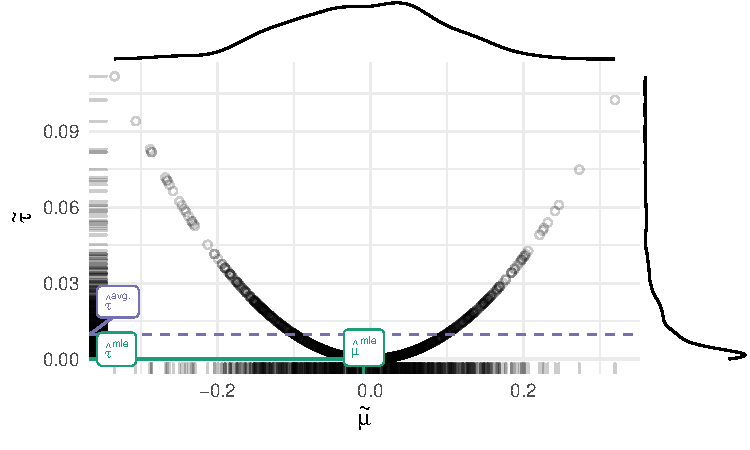
\includegraphics[width=.8\linewidth]{figs/intuition-1.pdf}
  \caption{Simulation 1 of 1,000}
  \label{fig:int1}
\end{subfigure}%
\begin{subfigure}{.5\textwidth}
  \centering
  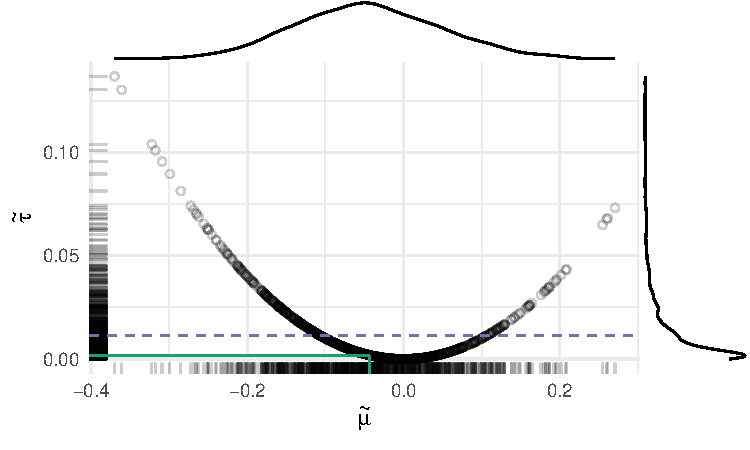
\includegraphics[width=.8\linewidth]{figs/intuition-2.pdf}
  \caption{Simulation 2 of 1,000}
  \label{fig:int2}
\end{subfigure}
\begin{subfigure}{.5\textwidth}
  \centering
  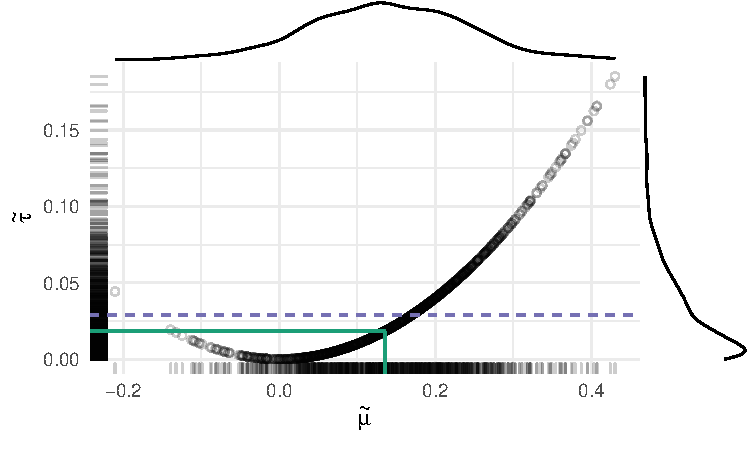
\includegraphics[width=.8\linewidth]{figs/intuition-3.pdf}
  \caption{Simulation 3 of 1,000}
  \label{fig:int3}
\end{subfigure}%
\begin{subfigure}{.5\textwidth}
  \centering
  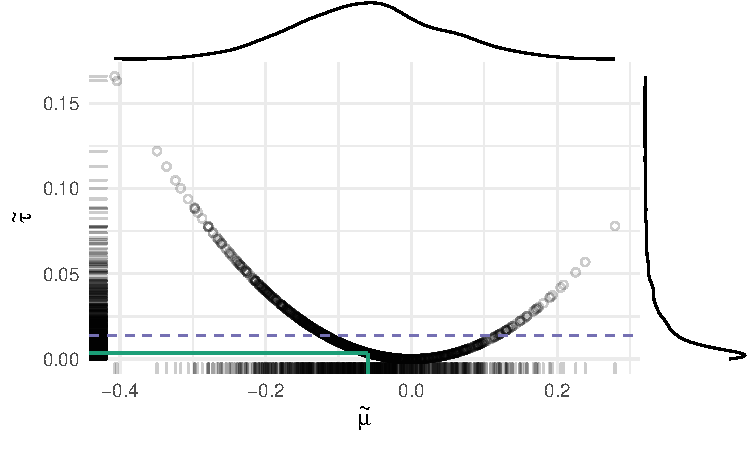
\includegraphics[width=.8\linewidth]{figs/intuition-4.pdf}
  \caption{Simulation 4 of 1,000}
  \label{fig:int4}
\end{subfigure}
\caption{Four figures illustrating the relationship between $\hat{\tau}^\text{mle}$ and $\hat{\tau}^\text{avg.}$ described by Lemma \ref{lem:direction} and Theorem \ref{thm:direction}.}
\label{fig:int}
\end{figure}

Second, to find $\hat{\tau}^\text{mle}$, we simply transform $\hat{\mu}^\text{mle}$ directly using $\hat{\tau}^\text{mle} = \left( \hat{\mu}^\text{mle} \right) ^2$. 
The solid, green lines show this transformation. 
Notice that $\hat{\tau}^\text{mle}$ corresponds to the mode of the density plot of $\tilde{\tau}$ along the right side of the plot, which falls closer to the true value $\tau(0) = 0$ than $\hat{\tau}^\text{avg.}$.
The convex transformation $\tau$ has the effect of lengthening the right tail of the distribution of $\tilde{\tau}$, which pulls the average well above the mode. 
This provides the basic intuition for Lemma \ref{lem:direction}.

Figures \ref{fig:int2}-\ref{fig:int4} repeat this process three more times to give some sense of how the dynamic changes for different data sets $y$.
In each case, the story is similar--the convex transformation $\tau$ stretches the distribution of $\tilde{\tau}$ to the right, which pulls $\hat{\tau}^\text{avg.}$ above $\hat{\tau}^\text{mle}$.

We repeat this process until we have 1,000 different estimates of $\hat{\mu}^\text{mle}$, $\hat{\tau}^\text{mle}$, and $\hat{\tau}^\text{avg.}$. 
Figure \ref{fig:int-samp} shows the density plot for each of these 1,000 estimates (i.e., the sampling distributions).
Notice $\hat{\mu}^\text{mle}$ is unbiased with a standard error of $\frac{1}{\sqrt{n}} = \frac{1}{\sqrt{100}} = \frac{1}{10}$.  
This confirms a basic result from statistical theory.
Both $\hat{\tau}^\text{mle}$ and $\hat{\tau}^\text{avg.}$ are biased upward, but $\hat{\tau}^\text{avg.}$ more so. 
Theorem \ref{thm:direction} ensures this must be the case. 

\begin{figure}[h]
\begin{center}
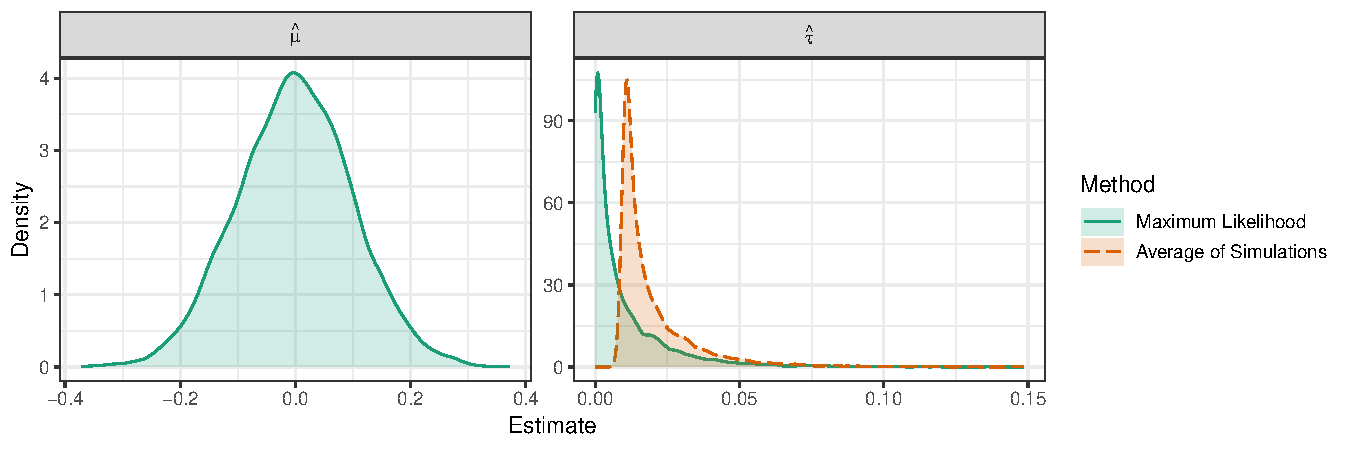
\includegraphics[scale = 0.6]{figs/intuition-sampling.pdf}
\caption{The sampling distributions of $\hat{\beta}^\text{mle}$, $\hat{\tau}^\text{mle}$, and $\hat{\tau}^\text{avg.}$.}\label{fig:int-samp}
\end{center}
\end{figure}

\subsection*{Using the Law of Iterated Expectations}

We can also develop the intuition using a more mathematical approach via the law of iterated expectations. 
However, it helps if we alter the notation slightly, making two implicit dependencies explicit. 
We explain each change below and use the alternate, more expansive notation only in this section.
 
The law of iterated expectations states that $\E_Y \left( \E_{X|Y}(X | Y) \right) = E_X(X)$, where $X$ and $Y$ represent random variables. 
The three expectations occur with respect to three different distributions: $\E_Y$ denotes the expectation w.r.t. the marginal distribution of $Y$, $\E_{X|Y}$ denotes the expectation w.r.t. the conditional distribution of $X | Y$, and $\E_X$ denotes the expectation w.r.t. the marginal distribution of $X$. 

Outside of this section, we realize that the distribution of $\tilde{\beta}$ depends on $\hat{\beta}^\text{mle}$ and could be written as $\tilde{\beta} | \hat{\beta}^\text{mle}$. 
To remain consistent with other papers, especially \cite{KingTomzWittenberg2000} and \cite{Herron1999}, we simply use $\tilde{\beta}$ to represent $\tilde{\beta} | \hat{\beta}^\text{mle}$.
The definition of $\tilde{\beta}$ makes this clear. 
In this section only, we use $\tilde{\beta} | \hat{\beta}^\text{mle}$ to represent the conditional distribution of $\tilde{\beta}$. 
we use $\tilde{\beta}$ to represent the \underline{un}conditional distribution of $\tilde{\beta}$.
Intuitively, one might imagine (1) generating a data set $y$, (2) estimating $\hat{\beta}^\text{mle}$, and (3) simulating $\tilde{\beta} | \hat{\beta}^\text{mle}$. 
If we do steps (1) and (2) just once, but step (3) repeatedly, then we have a sample from the conditional distribution $\tilde{\beta} | \hat{\beta}^\text{mle}$. 
If we do steps (1), (2), and (3) repeatedly, then we have a sample from the \underline{un}conditional distribution $\tilde{\beta}$. 
The unconditional distribution helps one understand the additional bias.\footnote{More technically, we could also define the relevant distributions hierarchically. First, we have $\hat{\beta}^\text{mle} \sim s(\beta)$, where $s(\beta)$ represents the sampling distribution of $\hat{\beta}$. Then we have $\tilde{\beta} \sim N \left[ \hat{\beta}^{\text{mle}}, \hat{V} \left( \hat{\beta}^{\text{mle}} \right) \right]$.}

Applying the law of iterated expectations, we obtain $\E_{\tilde{\beta}} \left( \tilde{\beta} \right) = \E_{\hat{\beta}^\text{mle}}\left( \E_{\tilde{\beta} | \hat{\beta}^\text{mle}} (\tilde{\beta} | \hat{\beta}^\text{mle}) \right)$.
%Using the law of the unconscious statistician, we have $\E_{\tilde{\beta}} \left( \tau \left[\tilde{\beta} \right] \right) = \E_{\hat{\beta}^\text{mle}}\left( \E_{\tilde{\beta}) | \hat{\beta}^\text{mle}} \left( \tau[\tilde{\beta}] | \hat{\beta}^\text{mle} \right) \right)$.
The three identities below connects the three key quantities from Theorem \ref{thm:direction} to three versions of $\E_{\hat{\beta}^\text{mle}}\left( \E_{\tilde{\beta} | \hat{\beta}^\text{mle}} (\tilde{\beta} | \hat{\beta}^\text{mle}) \right)$, with the transformation $\tau$ applied at different points.

\begin{alignat}{2}
 \color{color1} \tikzmark{MarkA}\tau \left[ \normalcolor \E_{\hat{\beta}^\text{mle}}\left( \E_{\tilde{\beta} | \hat{\beta}^\text{mle}} \left( \tilde{\beta} | \hat{\beta}^\text{mle} \right) \right) \color{color1} \right] \normalcolor =&  \tau \left[ \E_{\tilde{\beta}} \left( \tilde{\beta} \right) \right] = \tau \left[\E \left( \hat{\beta}^\text{mle} \right) \right]\text{,} \label{eqn:true}\\
 \E_{\hat{\beta}^\text{mle}}\left( \color{color1} \tikzmark{MarkB}\tau\tikzmark{MarkC} \left[ \normalcolor \E_{\tilde{\beta} | \hat{\beta}^\text{mle}} \left( \tilde{\beta} | \hat{\beta}^\text{mle} \right) \color{color1} \right] \normalcolor \right)  =&  \E_{\hat{\beta}^\text{mle}} \left( \tau \left[\hat{\beta}^\text{mle} \right] \right) =  \E_{\hat{\beta}^\text{mle}} \left(\hat{\tau}^\text{mle} \right) \text{, and} \justif{\quad}{$\longleftarrow~$ Switch $\tau$ and an $\E$ once.} \label{eqn:mle}\\
\E_{\hat{\beta}^\text{mle}}\left( \E_{\tilde{\beta} | \hat{\beta}^\text{mle}} \left( \color{color1} \tikzmark{MarkD}\tau \left[ \normalcolor \tilde{\beta} | \hat{\beta}^\text{mle} \color{color1} \right] \normalcolor \right) \right)  =& 
\E_{\tilde{\beta}} \left( \tau \left[\tilde{\beta} \right] \right)  = 
\E_{\tilde{\beta}} \left(\hat{\tau}^\text{avg.} \right) \text{.}\justif{\quad}{$\longleftarrow~$ Switch $\tau$ and an $\E$ again.}\label{eqn:avg}\DrawBox{red}{blue}
\end{alignat}

If we subtract Equation \ref{eqn:mle} from Equation \ref{eqn:true}, then we obtain the transformation-induced $\tau$-bias in $\hat{\tau}^\text{mle}$ (see Equation \ref{eqn:ti-bias} for the definition of transformation-induced $\tau$-bias). 
To move from Equation \ref{eqn:true} from Equation \ref{eqn:mle}, we must swap $\tau$ with an expectation once, so, if $\tau$ is convex, then Equation \ref{eqn:mle} must be greater than Equation \ref{eqn:true}.
This, in turn, implies that the bias is positive.

To obtain the transformation-induced $\tau$-bias in $\hat{\tau}^\text{avg}$, we must subtract Equation \ref{eqn:avg} from Equation \ref{eqn:true}. 
But to move from Equation \ref{eqn:true} from Equation \ref{eqn:avg}, we must swap $\tau$ with an expectation \emph{twice}. 
Again, if $\tau$ is convex, then Equation \ref{eqn:avg} must be greater than Equation \ref{eqn:true}.
However, because we expect $\hat{\beta}^\text{mle}$ and $\tilde{\beta} | \hat{\beta}^\text{mle}$ to have similar distributions, we should expect the additional swap to roughly double the bias in $\hat{\tau}^\text{avg.}$ compared to $\hat{\tau}^\text{avg.}$.

\section*{Illustrative Simulations}

\subsection*{Marginal Effects in Poisson Regression}

As an illustration, consider the Poisson regression model $y_i \sim \text{Poisson}(\lambda_i)$, where $\lambda_i = e^{(-2 + x_i)}$ for $i \in \{1, 2, ..., 100\}$. 
To create the $x_i$s, we simply took 100 draws from a standard normal distribution. 
Assume that the researcher wants to estimate the instantaneous marginal effect of $x$ on $\E(y)$ so that $\tau(\beta) = \frac{d \E (y)}{dx} = e^{(\beta_{cons} + \beta_x x)}$ for $x$ ranging from -3 to +3.

Following the procedures discussed above, we generate 10,000 data sets and use each data set to estimate $\hat{\tau}^\text{mle}$ and $\hat{\tau}^\text{avg.}$. 
Note that the transformation is convex, so Theorem \ref{thm:direction} guarantees that the transformation-induced $\tau$-bias in both $\hat{\tau}^\text{mle}$ and $\hat{\tau}^\text{avg.}$ will be positive. 
The rule of thumb suggests about twice as much bias in $\hat{\tau}^\text{avg.}$ as in $\hat{\tau}^\text{mle}$. 

Figure \ref{fig:poisson-mcs} shows the transformation-induced $\tau$-bias in $\hat{\tau}^\text{avg.}$ and $\hat{\tau}^\text{mle}$ compared to the true value $\tau(\beta)$. 
Especially notice three features of this plot. 
First, the bias is substantial. 
The relative size of the bias varies, but when the true marginal effect is greater than 0.5, the average transformation-induced $\tau$-bias in $\hat{\tau}^\text{mle}$ is about $\frac{1}{3}$ the size of the true effect. 
For $\hat{\tau}^\text{avg.}$, the bias is about $\frac{3}{4}$ the size of the true effect. 
Second, notice that the bias occurs in the expected direction. 
Because the transformation $\tau(\beta) = \frac{d \E (y)}{dx} = e^{(\beta_{cons} + \beta_x x)}$ is convex, the bias is positive. 
Third, notice that the bias in $\hat{\tau}^\text{avg.}$ is about twice as large as the bias in $\hat{\tau}^\text{mle}$, as the rule of thumb suggests.

\begin{figure}[h!]
\begin{center}
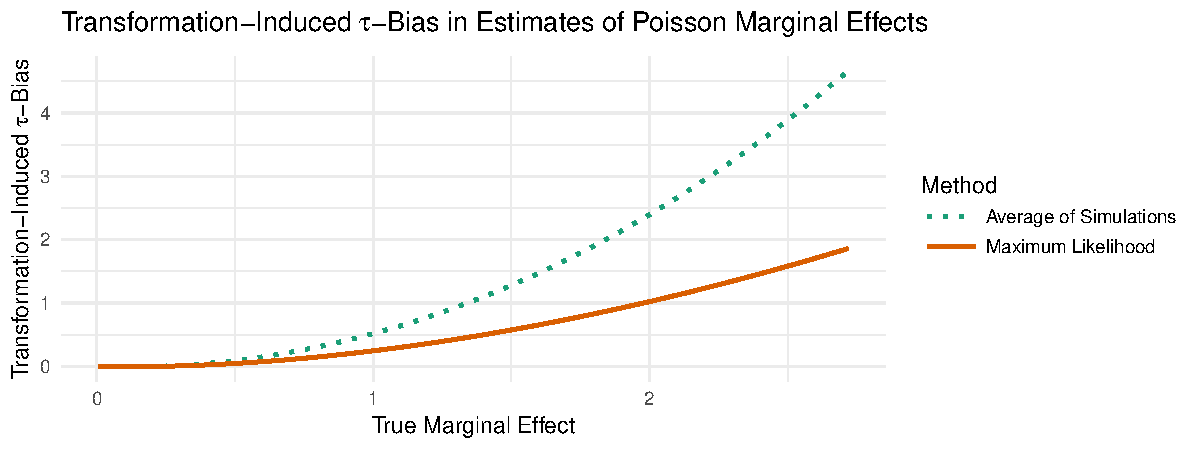
\includegraphics[scale = 0.6]{figs/poisson-mcs.pdf}
\caption{This figure shows the bias in the estimates of the marginal effects in a Poisson regression model. Notice that the convex transformation $\tau(\beta) = \frac{d \E (y)}{dx} = e^{(\beta_{cons} + \beta_x x)}$ creates a positive bias (see Theorem \ref{thm:direction}) and that the bias in $\hat{\tau}^\text{avg.}$ is about twice as large as the bias in $\hat{\tau}^\text{mle}$ (compare Equations \ref{eqn:avg-approx} and \ref{eqn:mle-approx}).}\label{fig:poisson-mcs}
\end{center}
\end{figure}

%\subsection*{Predicted Probabilities in Logistic Regression}
%
%When the quantity of interest is the marginal effect from a Poisson regression, we have an advantage: the transformation is strictly convex. 
%But many quantities of interest require a transformation that is neither strictly convex nor concave.
%For examples, the inverse-logit transformation researchers use to calculate predicted probabilities convex for inputs less than zero and concave for inputs greater than zero. 
%
%But Theorem \ref{thm:direction} offers some intuition about this case. 
%If the coefficients being transformed (either $\hat{\beta}^\text{mle}$ or $\tilde{\beta}$) lie mostly in a convex region, then the estimated quantity of interest is biased upward and the average of simulations is about twice as biased as the maximum likelihood estimates.

\section*{Example: Supreme Court Decisions}

To unify explanation of U.S. Supreme Court decisions, \cite{GeorgeEpstein1992} fit a single probit model that combines the legal and extralegal models of Court decision-making to a data set of 64 decisions. 
The authors model the probability of a conservative decision as a function of whether the Solicitor General filed an Amicus brief (SG = 1) or not (SG = 0) and 10 other explanatory variables. 
%Table \ref{tab:ge-coefs} provides the coefficient estimates.\footnote{I do not obtain identical coefficient estimates and standard errors, but the estimates are similar.} 
See \cite{GeorgeEpstein1992} for the more details of the model.

%\begin{table}
%\begin{center}
%\begin{tabular}{l c }
%\hline
% & Coef. (S.E.) \\
%\hline
%Intercept                                  & $-13.62 \; (3.60)^{*}$ \\
%Death-Qualified Jury                       & $1.28 \; (1.07)$       \\
%Capital Punishment Proportional to Offense & $2.96 \; (1.14)^{*}$   \\
%Particularizing Circumstances              & $1.14 \; (0.65)$       \\
%Aggravating Factors                        & $1.06 \; (0.67)$       \\
%State Psychiatric Examination              & $2.24 \; (0.88)^{*}$   \\
%Conservative Political Environment         & $2.18 \; (0.76)^{*}$   \\
%Court Change                               & $0.60 \; (0.38)$       \\
%State Appellant                            & $1.52 \; (0.74)^{*}$   \\
%Inexperienced Defense Counsel              & $1.08 \; (0.64)$       \\
%Repeat Player State                        & $1.89 \; (0.65)^{*}$   \\
%Amicus Brief from Solicitor General        & $1.79 \; (1.37)$       \\
%\hline
%Num. obs.                                  & 64                     \\
%\hline
%\multicolumn{2}{l}{\scriptsize{$^*p<0.05$}}
%\end{tabular}
%\caption{Statistical models}
%\label{tab:ge-coefs}
%\end{center}
%\end{table}

We use this model illustrate the potential impact of using the simulation average rather than the maximum likelihood estimate of the quantity of interest. 
We focus on two potential quantities of interest: the probability of a conservative decision and the effect of the Solicitor General filing a brief. 
Table \ref{tab:ge-qi} summarizes these quantities of interest. 

\begin{table}[h!]
\centering
\caption{This table provides the details of the quantities of interest from George and Epstein's (1992) model of U.S. Supreme Court decisions.}
\label{tab:ge-qi}
\footnotesize
\begin{tabular}{@{} m{5cm} m{4cm} m{2.5cm}m{4cm}@{}}
\toprule
Description                                                                       & Notation                                                  & Change in Key Explanatory Variable               & Values for Other Explanatory Variables \\ \midrule
probability of a conservative decision                                            & $\tau(\beta) = \Phi(X_c \beta)$                           & none                                             & every observed combination   \\\hline
effect of a Solicitor General brief on the probability of a conservative decision & $\tau(\beta) = \Phi(X_\text{high} \beta) - \Phi(X_\text{low}\beta)$ & for $X_\text{high}$, SG = 1, and for $X_\text{low}$, SG = 0 & every observed combination   \\ \bottomrule
\end{tabular}
\end{table}

For each quantity of interest, we compute an estimate using the average of simulation and maximum likelihood.
First, we use both the average of simulations and maximum likelihood to estimate the probability of a conservative decision for each combination of explanatory variables included in the data set. 
Second, we use both approaches to estimate the effect of a Solicitor General brief on the probability of a conservative decision. 
We define this effect as the \textit{difference} in the probability of a conservative decision for each observation in the data set, if that observation changed from one in which the Solicitor General \emph{did not} file a brief (SG = 0) to one in which the Solicitor General \emph{did} file a brief (SG = 1).

Figure \ref{fig:ge} compares the estimates. 
First, consider the estimates of the probability of a conservative decision in Figure \ref{fig:ge1}.
The pattern is clear: when the chance of a conservative decision is less than 50\%, the average of the simulations is too large. 
In this region, the transformation (the normal cdf) is convex. 
When the chance of a conservative decision is greater than 50\%, the average of the simulations is too small. 
In this region, the transformation is concave. 
When the chance of a conservative decision is closer to 50\%, the differences between the average of the simulations and the maximum likelihood estimate are smaller, because the transformation is more linear in this area. 
The same is true for chances close to 0\% and 100\%.

Further, some of the differences are quite large.
For example, when maximum likelihood suggests a chance of about 5\%, the average of the simulation suggests a chance of about 10\%. 
This difference may seem small at first (i.e., only 5 percentage points), but the average of simulations is about \textit{double} the maximum likelihood estimate. 


\begin{figure}[h!]
\begin{subfigure}{.5\textwidth}
  \centering
  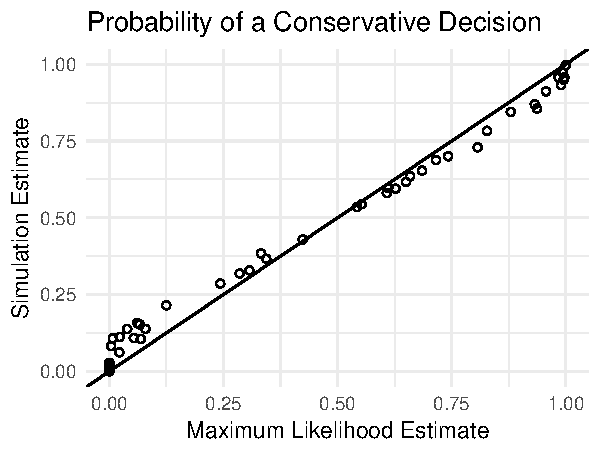
\includegraphics[width=.8\linewidth]{figs/ge-pr.pdf}
  \caption{}
  \label{fig:ge1}
\end{subfigure}%
\begin{subfigure}{.5\textwidth}
  \centering
  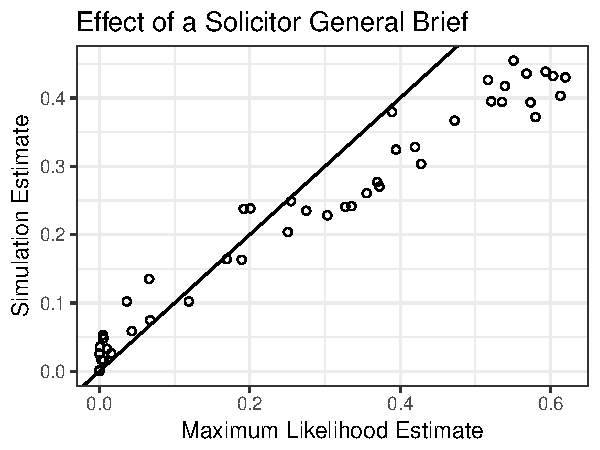
\includegraphics[width=.8\linewidth]{figs/ge-fd.pdf}
  \caption{}
  \label{fig:ge2}
\end{subfigure}
\caption{The figure shows the relationship between the simulation average and the maximum likelihood estimate two the quantities of interest. The left panel (a) shows the probability of a conservative decision. Notice that the simulation average tends falls about the maximum likelihood estimate when the probability is low--where the transformation is convex--and below the maximum likelihood estimate when the probability is high--where the transformation is concave. The right panel (b) shows the effect of a brief by the Solicitor General on the probability of a conservative decision.}
\label{fig:ge}
\end{figure}

Now consider the estimates of the effect of the Solicitor General filing an Amicus brief in Figure \ref{fig:ge2}.
The largest differences appear in the upper-right corner of the plot.
For this group of observations, the average of simulations suggests than a brief from the Solicitor General increases the chance of a conservative decision by about 40 percentage points. 
On the other hand, the maximum likelihood estimate suggests an increase of about 60 percentage points. 
This difference is certainly meaningful---the maximum likelihood estimate is 50\% larger than the average of the simulations.

\subsection*{A Note on \cite{HanmerKalkan2013}}

\cite{HanmerKalkan2013} discuss two approaches to computing quantities of interest: the typical ``average-case'' approach and their recommended ``observed-value'' approach. 
With either approach, the researcher estimates the quantity of interest--the change in the expected value of the outcome variable (e.g., the probability of a conservative decision) as a key explanatory variable changes from a low value to a high value (e.g., SG changes from 0 to 1). 
But the researcher must also deal with the other explanatory variables in the model, because these variables alter the quantity of interest. 
The average-case approach sets the other explanatory variables at a typical value, such as the median. 
\cite{HanmerKalkan2013} suggest estimating the quantity of interest for all the observed combinations of the other explanatory variables (like we do above) and then averaging the quantity of interest across the combinations. 
In our argument, this choice is built into the transformation $\tau$, so their (compelling) argument does not undermine or enhance our own.\footnote{We generally agree with their arguments in favor of the observed-value approach, but we recommend researchers plot the distribution of effects rather than summarizing them into a single average.} 
Because researchers have not drawn a sharp conceptual distinction between the simulation average and maximum likelihood estimates of the quantity of interest, \cite{HanmerKalkan2013} do not adopt a clear position. 
We read their paper to suggest averaging the maximum likelihood estimates ($\hat{\tau}^\text{mle}$) for each observed case (though they do not explicit write this). 
However, in their Stata code, they average the simulation averages ($\hat{\tau}^\text{avg.}$) for each observed case.

When we average the maximum likelihood estimates of the effect of a Solicitor General brief in the left panel (b) of Figure \ref{fig:ge} (as \cite{HanmerKalkan2013} seem to suggest in their paper), we obtain an estimated effect of 0.28. 
When we average the simulation averages (as Hanmer and Kalkan do in their Stata code), we obtain an estimated effect of 0.23. 
The maximum likelihood estimate is about 22\% larger than the simulation average--the choice matters.

The important point is this: \cite{HanmerKalkan2013} draw a distinction between the average-case and observed-value approaches to choosing the quantity of interest. 
This paper draws a distinction between estimating quantities of interest (whether average-case or observed-value) using the simulation average and the maximum likelihood estimate. 
Regardless of whether the researcher uses the average-case approach or the observed-value approach, the simulation average is more biased than the maximum likelihood estimate.

\section*{Conclusion}

Substantive researchers in political science tend to estimate their quantity of interest using the average of simulation (e.g., CLARIFY in Stata, Zelig in R) or using the invariance property of maximum likelihood estimates (e.g., margins in Stata). 
In practice, researchers' choice between the two seems idiosyncratic rather than principled. 
But the choice is clear. 
\cite{Rainey2017} introduces the idea of transformation-induced bias. 
This paper shows that the average of the simulations roughly \textit{doubles} this bias.
In many cases, the researcher has small standard errors. 
In this case, the additional bias is small. 
But in other cases, such as when the researcher has large standard errors or focuses on a highly non-linear transformation of the model coefficients, the bias is substantial. 
And the fix is easy: simply plug the coefficient estimates into the transformation to obtain the maximum likelihood estimates of the quantity of interest. 
Software should do this by default. 


\singlespace 
%\newpage
\small
\bibliographystyle{apsr_fs}
\bibliography{/Users/carlislerainey/Dropbox/papers/bibliography/bibliography.bib}

\end{document}


















